%% Ein einfaches Template für einen Übungsbericht unter Verwendung des Hagenberg
%% Setups, basierend auf der LaTeX 'report' Standardklasse.
%%% äöüÄÖÜß  <-- keine deutschen Umlaute hier? UTF-faehigen Editor verwenden!

%%% Magic Comments zum Setzen der korrekten Parameter in kompatiblen IDEs
% !TeX encoding = utf8
% !TeX program = pdflatex
% !TeX spellcheck = de_DE
% !BIB program = biber

\documentclass[german,notitlepage,smartquotes]{hgbreport}
% Zulässige Optionen in [..]:
%    Hauptsprache: 'german' (default), 'english'
%    Option zur Umwandlung in typografische Anführungszeichen: 'smartquotes'
%    APA Zitierstil: 'apa'
%    Erzeuge keine separate Titelseite: 'notitlepage'
%%%-----------------------------------------------------------------------------

\RequirePackage[utf8]{inputenc} % bei Verw. von lualatex oder xelatex entfernen!

\renewcommand{\chapter}[1]{} % Deaktiviere den \chapter Befehl
\graphicspath{{images/}}     % Verzeichnis mit Bildern und Grafiken
\bibliography{references}    % Biblatex-Literaturdatei (references.bib)
\ExecuteBibliographyOptions{backref=false} % Keine Rückreferenzen bei Quellen

%%%-----------------------------------------------------------------------------
\setcounter{chapter}{5}	% <----- Auf die Übungsnummer setzen
%%%-----------------------------------------------------------------------------

\author{Julian Jany}                        % Name
\title{BVA2 Fortgeschrittene Bildverarbeitung und -analyse -- SS 2022\\ % Name der Übung
				Übungsabgabe \arabic{chapter}}
\date{\today}

%%%-----------------------------------------------------------------------------
\begin{document}
%%%-----------------------------------------------------------------------------
\maketitle
%%%-----------------------------------------------------------------------------

\lstset{language=Java,
		basicstyle=\ttfamily\footnotesize,
		keywordstyle=\color{blue}\ttfamily,
		stringstyle=\color{red}\ttfamily,
		commentstyle=\color[rgb]{0,0.608,0.333}\ttfamily, % ForestGreen
		morecomment=[l][\color{magenta}]{\#}
}


%\begin{abstract}\noindent
%\ldots
%\end{abstract}

%%%-----------------------------------------------------------------------------

\section{Structure from Motion}

\subsection{Problembeschreibung}

Es soll mittels eines entsprechenden Tools ein Objekt durch "Structure from Motion" (auch bekannt als \texttt{Photogrammetry}) digital rekonstruiert werden.

\subsection{Lösungsbeschreibung}

\subsubsection{Aufnahme der Bilder}

Beim Aufnehmen der Bilder sind folgende Einstellungen der Kamera zu beachten:

\begin{itemize}
	\item niedriger \texttt{ISO} Wert (im besten Fall \texttt{Base-ISO}) zur Minimierung von Rauschen
	\item hohe Blendenzahl ($f$/$8.0$ - $f$/$14.0$) für eine möglichst hohe Tiefenschärfe
	\item Einsatz eines Stativs um Bewegungsunschärfe zu vermeiden
	\item gute Ausleuchtung des zu scannenden Objekts
	\item Aufnahme in \texttt{RAW} um Kompressionsartefakte zu vermeiden
\end{itemize}

Es werden bewussts einzelne Standbilder anstelle eines Videos aufgenommen; mit dem Hintergrund, temporale und räumliche Kompressionsartefakte zu vermeiden und so bessere Endresultate erzielen zu können.

\subsubsection{Vorverarbeitung}

Die aufgenommenen \texttt{RAW} Bilder werden in einem \texttt{RAW-Converter} vorverarbeitet. 
Abb. \ref{input_imgs} zeigt vier der insgesamt 69 zur Rekonstruktion aufgenommenen Bilder.

\begin{figure}[h]
	\centering\small
	\begin{tabular}{cc}
		\FramePic{\includegraphics[width=0.45\textwidth]{_DSF1534-1.png}} &
		\FramePic{\includegraphics[width=0.45\textwidth]{_DSF1537-1.png}} \\
		\FramePic{\includegraphics[width=0.45\textwidth]{_DSF1545-1.png}} &
		\FramePic{\includegraphics[width=0.45\textwidth]{_DSF1569-1.png}}
	\end{tabular}
	\caption{Ein Auszug der zur Rekonstruktion aufgenommenen Bilder.}
	\label{input_imgs}
\end{figure}

\clearpage

\subsection{Structure from Motion}

Zur Rekonstruktion wird das open-source Tool \href{https://alicevision.org/}{Meshroom} eingesetzt.

Im Folgenden werden alle Schritte zum Erstellen des 3D-Modells beschrieben.

\subsubsection{\texttt{CameraInit}}

Dieser Knoten beschreibt den Datensatz. Er listet die Viewpoint-Kandidaten, die Vermutung über die Art der Optik, die anfängliche Brennweite und die Bilder auf, die dieselben internen Kameraparameter haben, sowie mögliche Kamera-Rigs.

\subsubsection{\texttt{FeatureExtraction}}

Dieser Knotenpunkt extrahiert charakteristische Gruppen von Pixeln, die in gewissem Maße unabhängig von wechselnden Kamerastandpunkten während der Bildaufnahme sind.
Es stehen einige Feature-Extraktoren zur Auswahl, standardmäßig wird der \texttt{SIFT} verwendet.

\subsubsection{\texttt{ImageMatching}}

Die Aufgabe dieses Knoten ist es, Bilder zu finden, die die gleichen Bereiche der Szene zeigen.
Das Ziel dabei ist es, Bildpaare für den für das \texttt{FeatureMatching} auszuwählen.
Dank dieses Knotens wird der \texttt{FeatureMatching}-Knoten nur die Übereinstimmungen zwischen den ausgewählten Bildpaaren berechnen und so die Rechenzeit deutlich reduzieren.

\subsubsection{\texttt{FeatureMatching}}

Dieser Knoten iteriert über alle Kandidatenbildpaare und versucht möglichst viele Features eines Bildes den Features aus dem anderen Bild zuzuordnen.

\subsubsection{\texttt{StructureFromMotion}}

Dieser Knoten analysiert Merkmalsübereinstimmungen (Feature-Matches), um die geometrische Beziehung hinter allen 2D-Beobachtungen zu verstehen, und leitet die starre Szenenstruktur (3D-Punkte) mit der Pose (Position und Orientierung) und der internen Kalibrierung aller Kameras ab. Die Pipeline ist ein wachsender Rekonstruktionsprozess (genannt inkrementelles SfM): Sie berechnet zunächst eine anfängliche Rekonstruktion aus zwei Ansichten, die iterativ durch Hinzufügen neuer Ansichten erweitert wird.

\subsubsection{\texttt{PrepareDenseScene}}

Dieser Knoten exportiert unverzerrte Bilder, damit die Depthmap und die Texturierung auf "Pinhole-Bildern" ohne Verzerrung berechnet werden können.
Im Idealfall werden bereits kalibrierte Bilder als Input verwendet und dieser Knoten sollte nur minimale Korrekturen vornehmen.

\subsubsection{\texttt{DepthMap}}

Für jede Kamera, die mittels Structure from Motion ermittelt wird, schätzt dieser Knoten den Tiefenwert pro Pixel.

\subsubsection{\texttt{DepthMapFilter}}

Filtert Depthmap-Werte, die in mehreren Depthmaps nicht kohärent sind.
Dadurch können instabile Punkte gefiltert werden, bevor die Fusion aller Depthmaps im Meshing-Knoten gestartet wird.

\subsubsection{\texttt{Meshing}}

Dieser Knoten erstellt eine dichte geometrische Oberflächendarstellung der Szene.
Zunächst werden alle Depthmaps zu einer globalen dichten Punktwolke mit einer adaptiven Auflösung verschmolzen. Anschließend wird eine 3D-Delaunay-Tetraederisierung durchgeführt und ein Abstimmungsverfahren zur Berechnung der Gewichte für die Zellen und der Gewichte für die Facetten, die die Zellen verbinden, angewandt. Ein Graph Cut Max-Flow wird angewendet, um das Volumen optimal zu schneiden. Dieser Schnitt stellt die extrahierte Netzoberfläche dar.

\subsubsection{\texttt{MeshFiltering}}

Dieser Knoten wendet eine Laplacian-Filterung an, um lokale Defekte aus dem Meshing-Rohschnitt zu entfernen.

\subsubsection{\texttt{Texturing}}

Dieser Knoten berechnet die Texturierung des Meshes.
Wenn das Mesh keine zugehörige UV hat, berechnet er automatisch UV-Maps.
Für jedes Dreieck verwendet er die Sichtbarkeitsinformationen, die mit jedem Scheitelpunkt verbunden sind, um die Texturkandidaten zu finden. Es wählt die besten Kameras auf der Grundlage der das Dreieck abdeckenden Auflösung aus. Schließlich werden die Pixelwerte unter Verwendung mehrerer Bänder im Frequenzbereich gemittelt. Viele Kameras tragen zu den niedrigen Frequenzen bei und nur die besten tragen zu den hohen Frequenzen bei.



\clearpage

\subsection{Ergebnis}

\begin{figure}[h]
	\centering\small
	\begin{tabular}{c}
		\FramePic{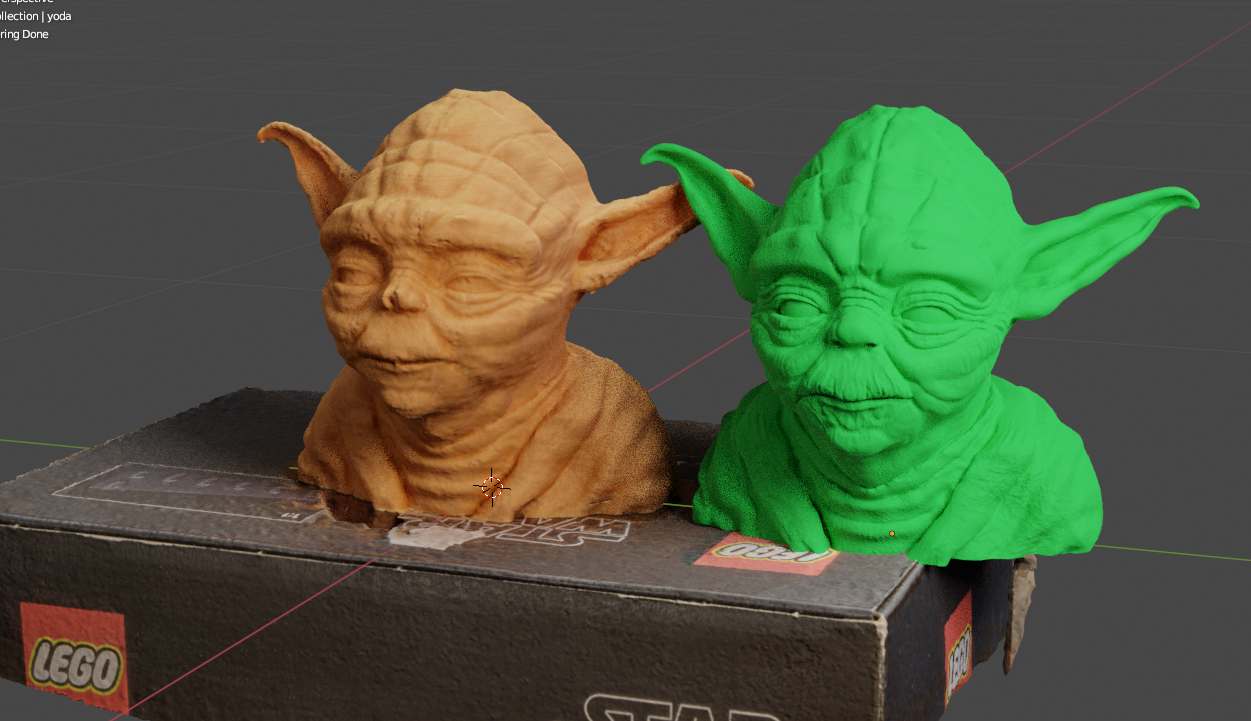
\includegraphics[width=0.7\textwidth]{reconstructed_05_comparison.png}} \\
		\FramePic{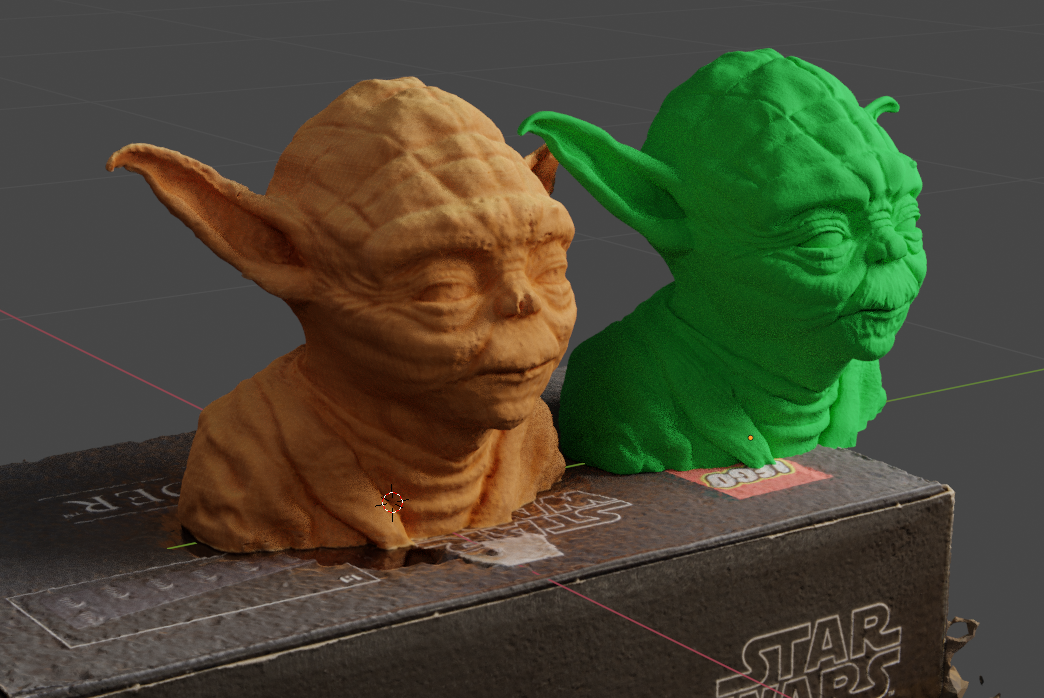
\includegraphics[width=0.7\textwidth]{reconstructed_06_comparison.png}}
	\end{tabular}
	\caption{Zwei Perspektiven welche jeweils das digitale Ausgangsmodell (grün) und des rekonstruierte Modell (orange) zeigen.}
	\label{example02}
\end{figure}

\begin{figure}[h]
	\centering\small
	\begin{tabular}{cc}
		\FramePic{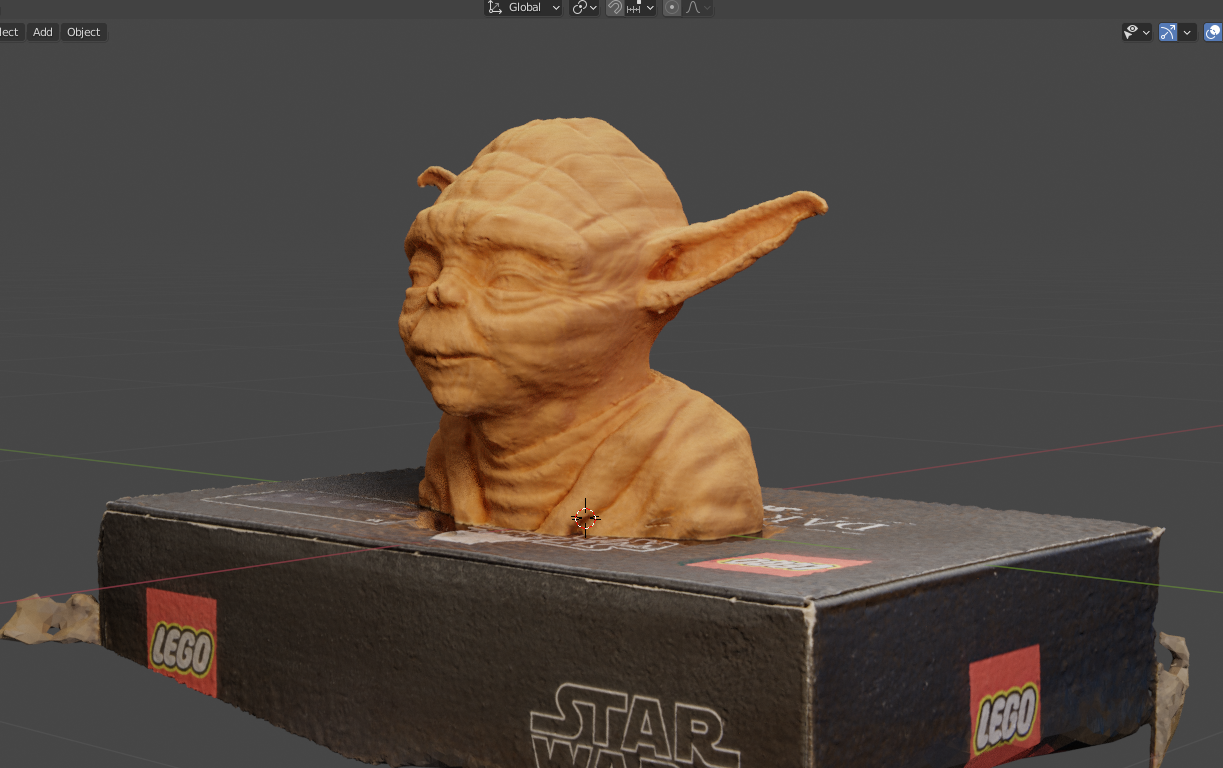
\includegraphics[width=0.45\textwidth]{reconstructed_01.png}} &
		\FramePic{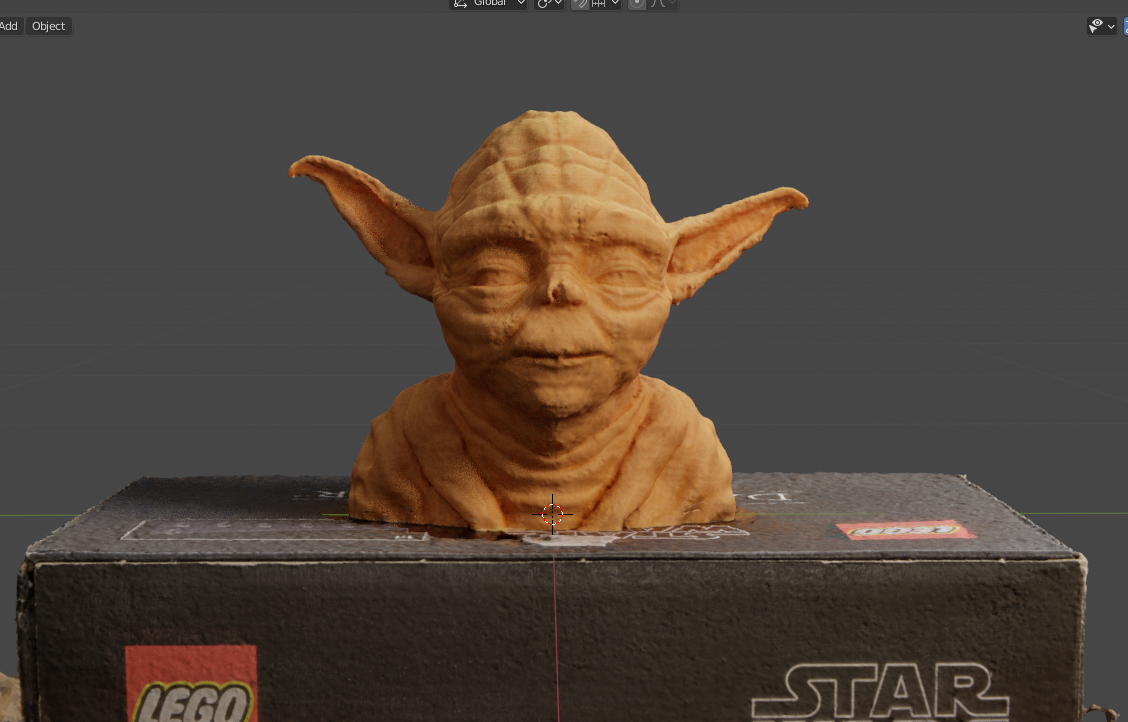
\includegraphics[width=0.45\textwidth]{reconstructed_02.png}} \\
		\FramePic{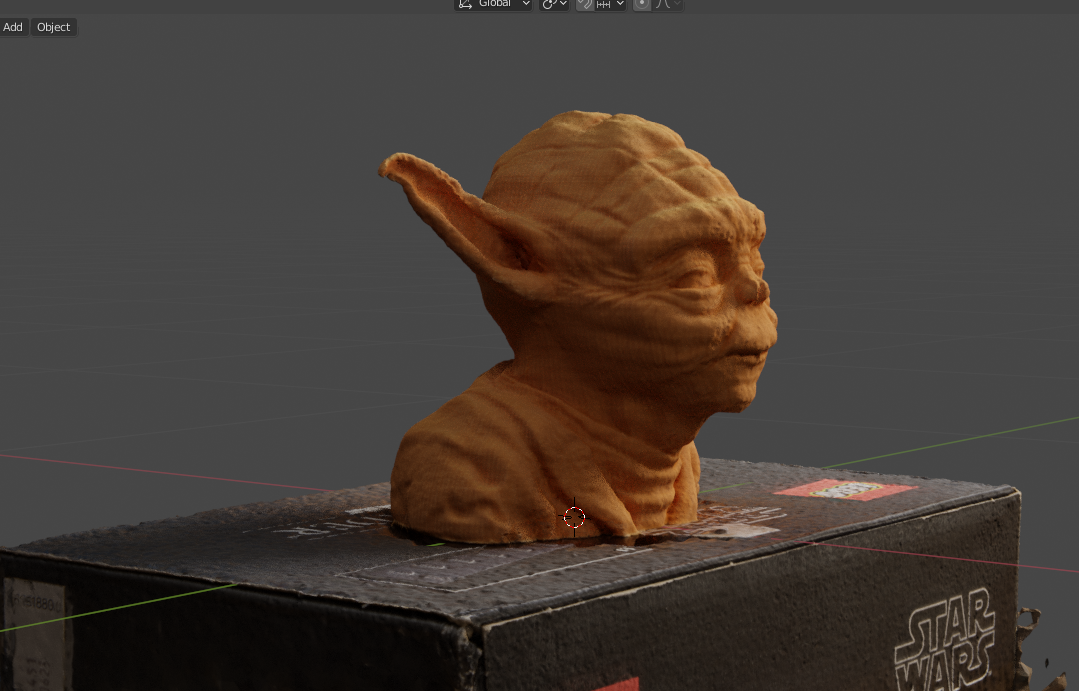
\includegraphics[width=0.45\textwidth]{reconstructed_03.png}} &
		\FramePic{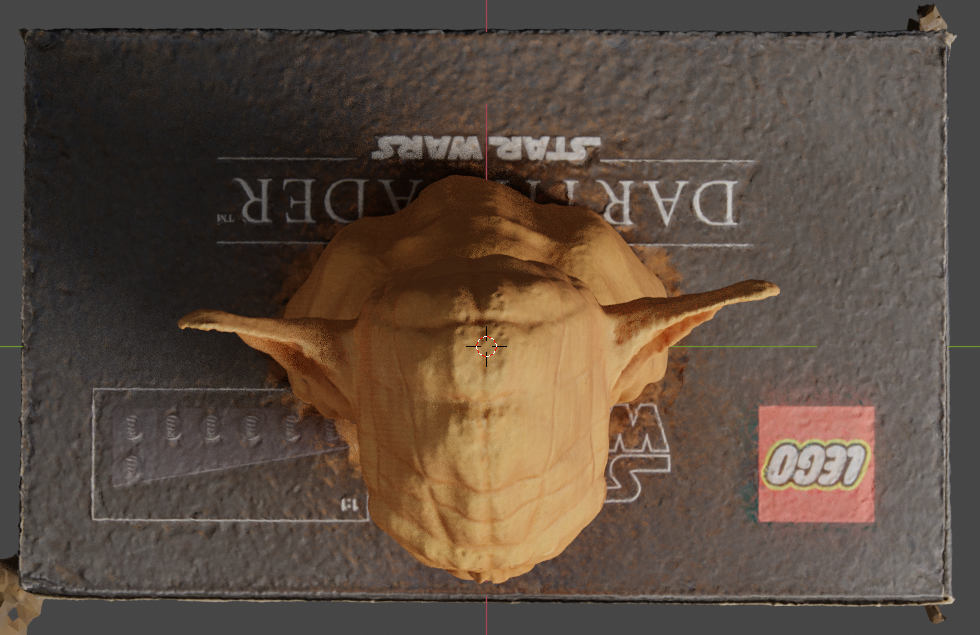
\includegraphics[width=0.45\textwidth]{reconstructed_04.png}}
	\end{tabular}
	\caption{Mehrere Perspektiven welche jeweils das rekonstruierte Modell zeigen.}
	\label{example01}
\end{figure}

% ---------------------------------------------------------------

\clearpage

\subsection{Erkenntnisse}

Die Parameter haben teils einen sehr großen Einfluss auf die Qualität der Ergebnisse. Mit gut gewählten Parametern können "erstaunlich" gute Rekonstruktionen realisiert werden, vorallem für einen -- zumindest in der Implementierung -- simplen Algorithmus.

%%%-----------------------------------------------------------------------------

% \section{Titel der zweiten Aufgabe}

%%%-----------------------------------------------------------------------------

%\section*{Zusammenfassung und Anmerkungen}

%%%-----------------------------------------------------------------------------

% \section*{Quellen}

% \printbibliography[heading=noheader]

%%%-----------------------------------------------------------------------------
\end{document}
%%%-----------------------------------------------------------------------------